\chapter{Implementation of Species Transport }\label{ch:implimentation_of_species_transport}

Implementing the generalized multi-phase species transport equation is done on a finite volume mesh. Each cell volume is integrated over and all properties and scalar quantities are assumed to be constant in the cell. Because the entire cell volume is integrated, species concentration are solved for concentration changes in the cell volume and not the phase volume. This treatment requires that volumetric source terms be integrated over the phase volume and not the cell volume to ensure that mass is conserved. 

% Averaging operators
\section{Averaging Operators}
Various methods of averaging exist for converting microscopic conservation equations into macroscopic ones. This technique involves averaging parameters of interest over space, time or both where the spacial variation of concentration is ignored in the cell. CTF is discritized on a finite volume mesh, meaning that volume averaging operators will be needed for species concentration for all phases in the unit cell. Let \textit{V} represent total volume of a cell, \textit{V} can be broken up further into sub domains \textit{$V_{l}$} and \textit{$V_{g}$} where \textit{l} denotes liquid and \textit{g} denotes gas. The volume average of species concentration \textit{C} over the entire volume is shown in Equation \ref{eq:avg_op_over_cell} \cite{kazimi1990}:

\begin{equation}
    \overline{C} = \frac{1}{V}\iiint_{V}CdV
    \label{eq:avg_op_over_cell}
\end{equation}

The concentration can also be averaged over the phase volume \textit{k}:

\begin{equation}
    \overline{C}_{k} = \frac{1}{V_{k}}\iiint_{V_{k}}CdV = \frac{1}{V_{k}}\iiint_{V}\alpha_{k}CdV
    \label{eq:avg_spec_con}
\end{equation}

Where $\alpha_{k}$ is the phase density function; equal to 1 for a point in phase \textit{k} and zero when not. The fraction of cell volume occupied by phase \textit{k} is the void fraction $\overline{\alpha}_{k}$.

\begin{equation}
    \overline{\alpha}_{k} = \frac{1}{V}\iiint_{V}\alpha_{k}dV = \frac{V_{k}}{V}
    \label{eq:avg_void}
\end{equation}

The concentration of species in phase k can also be averaged over the volume occupied by phase k: this value is denoted by $\langle \overline{C}_{k} \rangle_{k}$. 

\begin{equation}
    \langle \overline{C}_{k} \rangle_{k} = \frac{1}{V_{k}}\iiint_{V_{k}}C_{k}dV = \frac{1}{V_{k}}\iiint_{V}\alpha_{k}C_{k}dV
    \label{eq:avg_spec_con_volk}
\end{equation}

Combining Equations \ref{eq:avg_spec_con}, \ref{eq:avg_void} and \ref{eq:avg_spec_con_volk} gives the relations between averaged concentrations.

\begin{equation}
    \overline{C}_{k} = \langle \overline{C}_{k} \rangle_{k}\overline{\alpha}_{k}
\end{equation}

The value $\langle \overline{C}_{k} \rangle_{k}$ represents the species concentration if all of the cell volume was occupied by phase k. $\overline{C}_{k}$ is the species concentration of interest. Multiplying $\overline{C}_{k}$ by \textit{V} returns the amount of species in the cell volume. 

% discretization
\section{Discretization}

%\subsection{Finite volume method}
Species transport utilizes the same discretization method as CTF, finite volume. The data types are further broken down in to scalar and vector (momentum) cells, with these cells overlapping one another shown in Figures \ref{fig:ax_mesh} and \ref{fig:lat_mesh} \cite{salko2017}. 

The averaged operators previously discussed are now applied to Equation \ref{eq:two_phase_species_con_integral_volume}; starting with the conservation of species \textit{i} in phase \textit{k}. 

\begin{equation}
	\iiint_{V} \frac{\partial \alpha_{k}C^{k}_{i} }{\partial t}\,dV = -\iint_S n \cdot F^{k}_{i} \,dS + \iiint_V \alpha_{k}C_{V,i}^{i} \,dV
	\label{eq:start_eq_of_discretization}
\end{equation}
\FloatBarrier
\newpage

\begin{figure}[p]
  \centering
  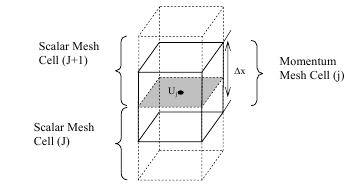
\includegraphics[width=4in]{images/axial_mesh_cells.png}\\
  \caption{Axial meshing.}
  \label{fig:ax_mesh}
\end{figure} 

\begin{figure}[p]
  \centering
  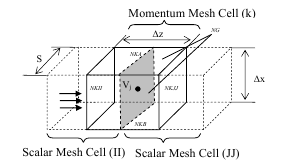
\includegraphics[width=4in]{images/lat_mesh_cells.png}\\
  \caption{Lateral meshing.}
  \label{fig:lat_mesh}
\end{figure} 

\newpage
\FloatBarrier

Starting with Equation \ref{eq:avg_spec_con_volk}, the time variance in equation \ref{eq:start_eq_of_discretization} is averaged over the cell volume to give:

\begin{equation}
    \iiint_{V} \frac{\partial \alpha_{k}C^{k}_{i} }{\partial t}\,dV = \frac{\partial V_{k}\langle \overline{C^{k}}_{i} \rangle_{k}}{\partial t}
\end{equation}

$V_{k}$ however, is $\overline{\alpha}_{k}V$ and $\langle \overline{C^{k}}_{i} \rangle_{k}\overline{\alpha}_{k} = \overline{C^{k}}_{i}$. This same relation is used to evaluate the second term on the left hand-side of Equation \ref{eq:start_eq_of_discretization}. Because the volume of each cell is constant, \textit{V} can be taken out of the time derivative and moved to the right hand side. 

\begin{equation}
    \frac{\partial \overline{C^{k}}_{i}}{\partial t} = - \frac{1}{V}\iint_S n \cdot F^{k}_{i} \,dS + \sum \overline{C^{k}}_{V,i}
    \label{eq:avg_transport_eqn}
\end{equation}

A summation is taken for the volumetric generation term to account for multiple source terms. 

% Upwind flux
\subsection{Upwind Differencing Scheme}
The contribution due to species flux across the cell boundary is modeled using an first order upwind differencing scheme \cite{versteeg2007}. This flux is convection dominate which allows for the removal of the diffusive term. The inner product of the unit normal flux across the face reduces to the velocity across the face multiplied by the species concentration in the neighboring cell or the cell itself, depending upon the flow direction. An example for 2-D flow is shown in Figure \ref{fig:upwind_difference_scheme} for scalar cell (i, j). 

In Figure \ref{fig:upwind_difference_scheme}, flow is going from left to right and bottom to up. When CTF loops over cell (i, j), it loops over all cells connected to calculate the flux across the cell faces. To calculate the inward flux, the velocity at the South and West faces are multiplied by the species concentration in cells (i-1, j) and (i, j-1). The outward flux from cell (i, j) is calculated by multiplying the species concentration is cell (i, j) by the velocity at each face. Because CTF works on a staggered mesh, the velocities at each cell face is defined at that location via the momentum mesh cells. For generalized 3-D flow on a Cartesian rectangular mesh, species flux is represented in Equation \ref{eq:integral_to_flux}.

\FloatBarrier
\newpage

\begin{figure}[p]
  \centering
  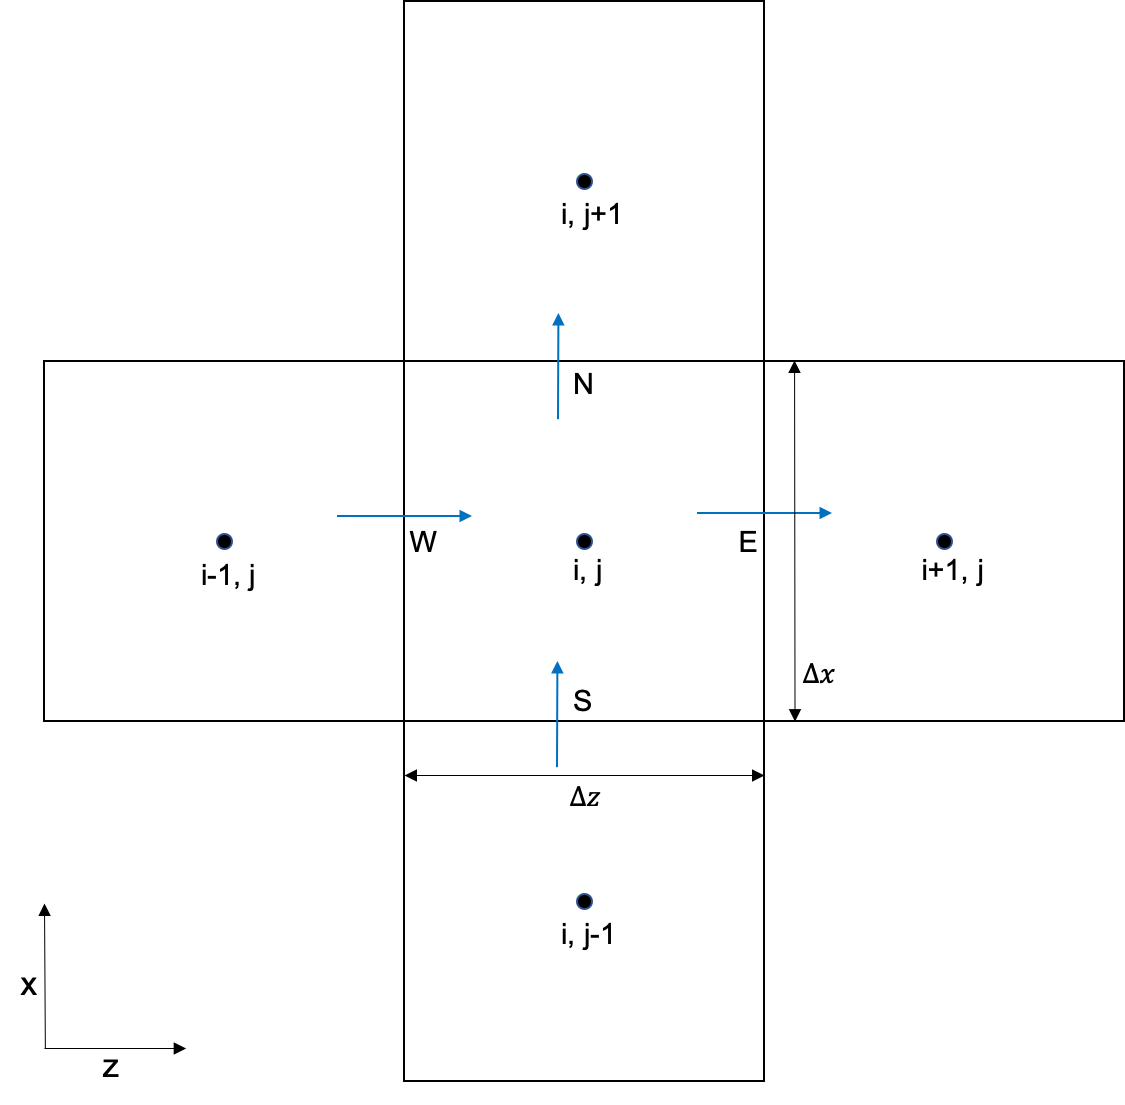
\includegraphics[width=4in]{images/2-DConvection.png}\\
  \caption{2-D Upwind flux}
  \label{fig:upwind_difference_scheme}
\end{figure}

\newpage
\FloatBarrier

\begin{equation}
    \frac{1}{V}\iint_S n \cdot F \,dS = \frac{1}{V}\bigg[ F_{x}A_{x} + F_{y}A_{y} + F_{z}A_{z}\bigg]
    \label{eq:integral_to_flux}
\end{equation}

Looking at Figure \ref{fig:upwind_difference_scheme} let us now define the positive z flow going from left to right, positive x flow going from down to up. Let's now add another dimension $y$, using $k$ index, pointing into the figure making the positive flow direction going into the page. The face coming out of the page is denoted by $O$ and in by $I$. $A_{x}$ becomes $\Delta z \Delta y$, $A_{z}$ becomes $\Delta x \Delta y$, $A_{y}$ becomes $\Delta x \Delta z$ and $V$ becomes $\Delta z \Delta x \Delta y$. If flow is assumed to be going to in the positive direction for each spacial degree of freedom, the flux for each direction is summarized in Table \ref{tab:upwind_flux_eqns}. 

In the case of 3-D flow in the positive direction, Equation \ref{eq:avg_transport_eqn} for a one species in single phase flow becomes:

\begin{equation}
\begin{aligned}
    \frac{\partial \overline{C}}{\partial t} = - \frac{1}{\Delta z \Delta x \Delta y}
     \bigg[ & \big(v_{S} \overline{C}_{i,j-1,k} - v_{N}\overline{C}_{i,j,k}\big)\Delta z \Delta y \\ + 
    & \big(v_{W} \overline{C}_{i-1,j,k} - v_{E}\overline{C}_{i,j,k}\big)\Delta x \Delta z \\ + 
    & \big(v_{O} \overline{C}_{i,j,k-1} - v_{I}\overline{C}_{i,j,k}\big)\Delta x \Delta y \bigg] + \sum \overline{C}_{V}
    \label{eq:avg_transport_eqn_with_flux}
\end{aligned}
\end{equation}

\subsection{Time Marching Scheme}
After discretizing the spacial variables of Equation \ref{eq:avg_transport_eqn}, the variance in time is addressed using two schemes: explicit and implicit Euler methods. For explicit methods, the time dependent solution is updated using information from the previous time step. Implicit methods utilize information on the current time step to solve the PDE. 

\vspace{12.7mm} %5mm vertical space

\begin{table}[htbp!]
   \caption{\label{tab:upwind_flux_eqns} Upwind flux}
   \centering
   \begin{tabular}{l l l}
   \hline
   \textbf{Flux} & \textbf{Positive flow} & \textbf{Negative flow} \\
   \hline 
    $F_{x} \approx$ & $v_{S} C_{i,j-1,k} - v_{N}C_{i,j,k}$ & $v_{N}C_{i,j,k} - v_{S} C_{i,j-1,k}$ \\ [1ex]
    $F_{y} \approx$ & $v_{W} C_{i-1,j,k} - v_{E}C_{i,j,k}$ & $v_{E}C_{i,j,k} - v_{W} C_{i-1,j,k}$ \\ [1ex]
    $F_{z} \approx$ & $v_{O} C_{i,j,k-1} - v_{I}C_{i,j,k}$ & $v_{I}C_{i,j,k} - v_{O} C_{i,j,k-1}$ \\ [1ex]
   \hline
   \end{tabular}
\end{table}

\subsubsection{Explicit Euler}
To derive the first order explicit Euler scheme we will start with Equation \ref{eq:avg_transport_eqn_with_flux} for 1-D flow in the x-direction.

\begin{equation}
        \frac{\partial \overline{C}}{\partial t} = - \frac{1}{\Delta x} \big(v_{S} \overline{C}_{j-1} - v_{N}\overline{C}_{j}\big)  + \sum \overline{C}_{V}
        \label{eq:1-D_x-direction_convection}
\end{equation}

The fundamental theorem of calculus states that the derivative of $\overline{C}(t,x)$ with respect to time is:

\begin{equation}
    \frac{\partial \overline{C}}{\partial t} = \lim_{\Delta t\to 0} \frac{\overline{C}(t+\Delta t, x) - \overline{C}(t,x)}{\Delta t}
    \label{eq:Def_theo_of_calc}
\end{equation}

Equation \ref{eq:Def_theo_of_calc} can be approximated by taking small values of $\Delta t$. Plugging in Equation \ref{eq:Def_theo_of_calc} into equation \ref{eq:1-D_x-direction_convection} and solving for $\overline{C}(t+\Delta t, x)$ gives:

\begin{equation}
    \overline{C}(t+\Delta t, x) = \overline{C}(t,x) - \frac{\Delta t}{\Delta x} \big(v_{S} \overline{C}_{j-1}(t,x) - v_{N}\overline{C}_{j}(t,x)\big)  + \Delta t\sum \overline{C}_{V}(t,x)
    \label{eq:explicit_method}
\end{equation}

% Consider moving this section
%%%%%%%%%%%%%%%%%%%%%%%%%%%%%%%%%%%%%%%%%%%%%%%%%%%%%%%%%%%%%%%%%%%%%%%%%
As previously mentioned, the upwind difference scheme is first order. The first order convergence is shown using a Taylor series expansion \cite{versteeg2007} for a simple 1-D example shown in Figure \ref{fig:1_D_upwind_flux}.

\begin{figure}[ht]
  \centering
  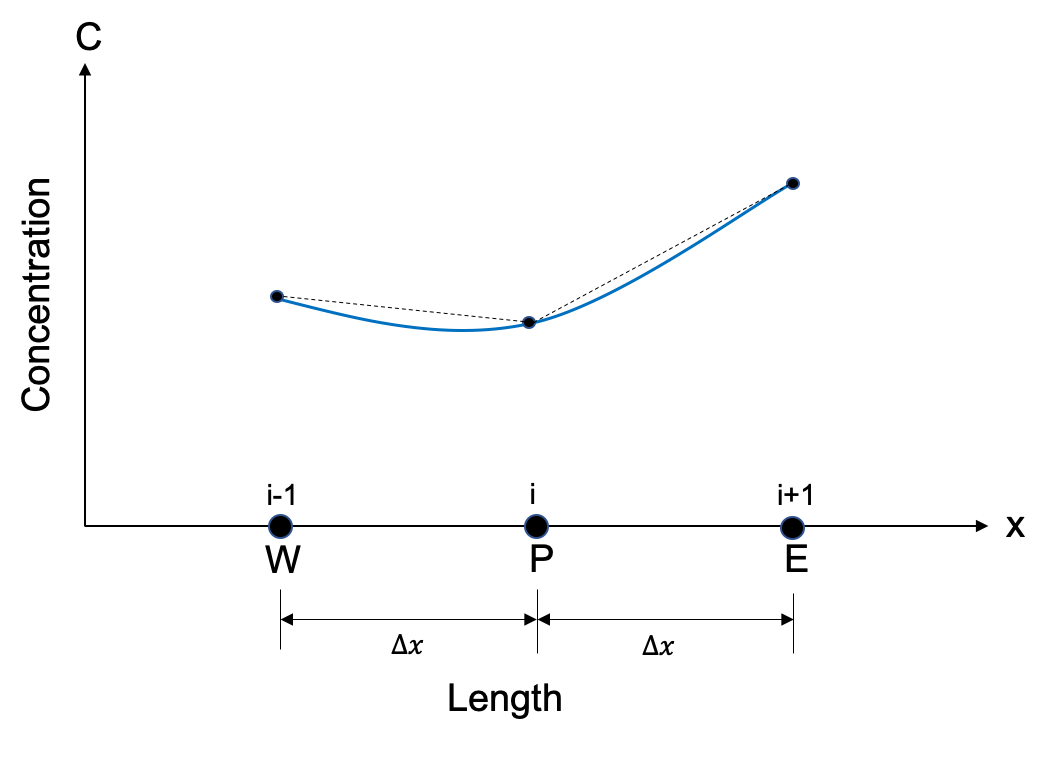
\includegraphics[width=5in]{images/1-DConvection.png}\\
  \caption{1-D Upwind flux}
  \label{fig:1_D_upwind_flux}
\end{figure}

For function $C(x + \Delta x)$ a Taylor series expansion about point $i$ at $x$ is shown in Equation \ref{eq:Taylor_second_order}.

\begin{equation}
    C(x+\Delta x) = C(x) + \bigg(\frac{\partial C}{\partial x}\bigg)_{x}\Delta x + \bigg(\frac{\partial^{2} C}{\partial x^{2}}\bigg)_{x}\frac{\Delta x^{2}}{2} + O(\Delta x^{3})
    \label{eq:Gen_Taylor_second_order}
\end{equation}

The concentration at Point $E$ (i+1) upwind of $P$ (i) is represented by Equation \ref{eq:Gen_Taylor_second_order}.

\begin{equation}
    C_{E} = C_{P} + \bigg(\frac{\partial C}{\partial x}\bigg)_{P}\Delta x + \bigg(\frac{\partial^{2} C}{\partial x^{2}}\bigg)_{P}\frac{\Delta x^{2}}{2} + O(\Delta x^{3})
    \label{eq:Taylor_second_order}
\end{equation}

Solving Equation \ref{eq:Taylor_second_order} for the first derivative gives:

\begin{equation}
    \bigg(\frac{\partial C}{\partial x}\bigg)_{P} = \frac{C_{E} - C_{P}}{\Delta x} - \bigg(\frac{\partial^{2} C}{\partial x^{2}}\bigg)_{P}\frac{\Delta x}{2} + ...
    \label{eq:Taylor_series_updwind_flux_order}
\end{equation}

Equation \ref{eq:Taylor_series_updwind_flux_order} shows that the derivative at point $P$ can be approximated by Equation \ref{eq:upwind_flux_approx} by truncating the higher order terms. 

\begin{equation}
    \bigg(\frac{\partial C}{\partial x}\bigg)_{P} \approx \frac{C_{E} - C_{P}}{\Delta x}
    \label{eq:upwind_flux_approx}
\end{equation}

The error involved in approximating the derivative is proportional to the size of $\Delta x$. This implies that the error in Equation \ref{eq:upwind_flux_approx} can be reduced by decreasing $\Delta x$ \cite{versteeg2007}. The rate at which the error approaches zero is then proportional to $\Delta x$ to the first power, making the scheme first order in space. 

For an implicit solution terms in Equation \ref{eq:explicit_method} are taken from the current time step.

\begin{equation}
    \overline{C}(t+\Delta t, x) = \overline{C}(t,x) - \frac{\Delta t}{\Delta x} \big(v_{S} \overline{C}_{j-1}(t+\Delta t,x) - v_{N}\overline{C}_{j}(t+\Delta t,x)\big)  + \Delta t\sum \overline{C}_{V}(t+\Delta t,x)
    \label{eq:implicit_method}
\end{equation}

The solution to Equation \ref{eq:implicit_method} is accomplished by solving a set of linear algebraic equations. 
%%%%%%%%%%%%%%%%%%%%%%%%%%%%%%%%%%%%%%%%%%%%%%%%%%%%%%%%%%%%%%%%%%%%%%%%%

